%--------------------------------------------------------------------------------
\chapter{LCS Hardware Module Design}

So far we covered the general concepts, messages, protocols as well as the LCS core library and a glimpse how all of this might be used. Let's take a break from all that concepts and mostly software talk. For the LCS core layers and the node firmware to run, hardware modules need to be built. Welcome to the next big part of this book. Here, we will talk about the LCS hardware modules. A hardware module conceptually consist of three key parts.

\begin{itemize}
\item communication
\item controller
\item function block(s)
\end{itemize}

At the center of a hardware module is the \textbf{controller}. There is a great variety of controllers and development environments available. When selecting a controller for LCS, we will talk in a minute which one was picked, its is important that there is enough CPU power and equally important a powerful development environment. A console command line interface and interfaces to load the software is also very handy for configuring, monitoring and debugging. The \textbf{communication} part implements at a minimum the LCS message bus interface for the messages to transmit between the modules. Finally, the \textbf{function block}s implement the hardware module specific capabilities.

 This chapter is the first in series of chapters on hardware modules. Instead of presenting complete schematics for each major hardware module, such as the base station, we will go a slightly different route. We will first present the basic components an LCS node might need. Definitively we will need a controller and a CAN bus interface. Some LCS nodes might make use of an extended non-volatile storage, others need plenty of digital outputs. Just like Lego Blocks, all these parts should be combined easily to form the desired LCS hardware module. We will tackle each component one at a time to understand how they work. The later chapters will just combine these basic blocks with minor adaptations and perhaps some very dedicated components for their functionality.

\section{Selecting the controller}

The module designs described in this book initially used the AtMega controller platform along with the Arduino IDE to write the software. There is the Arduino IDE and by now a whole set of different processors. Since it was released, the Atmega controller family and boards such as Arduino UNO, Arduino NANO, Arduino MEGA are in widespread use. The LCS core library program and non-volatile storage requirements do place however a higher demand on the controller capabilities.

Meanwhile, the Raspberry PI Pico \texttt{(PICO)} controller joined the club. And it has a lot to offer. The PICO is a dual core controller running at up to 200 Mhz. It features a whopping 16Mbytes of flash and 264 Kbytes of main memory. There are plenty of IO ports, and functional blocks for UARTs, SPI and I2C interfaces. What makes this controller especially interesting are the programmable PIO state machines that allow for implementing your own I/O protocols. For example, there is CAN bus software library \texttt{(can2040)} built using these state machines. This way no extra CAN bus controller is needed. The PICO comes with its own software development kit and also an Arduino IDE integration is available.

As time goes by, there will be for sure other capable controller entering the market. However, when you want to complete a project versus chasing the latest controllers, you will need to pick. In our case, the PICO is the controller of choice. Its capabilities match our requirements and will be a good choice for the years to come. nevertheless, the LCS library software should be designed as independent of a particular controller as possible. More on this later. 

\section{The Controller Platform}

 The following table gives some guidance on the capabilities needed in our designs. This list also applies in general to other controllers.

\begin{longtable}{@{}p{0.25\linewidth}p{0.6\linewidth}@{}}
    \caption{Controller Attributes} \\
    \toprule
    \textbf{Attributes} & \textbf{Notes} \\
    \midrule
    \endfirsthead
    \toprule
    \textbf{Attributes} & \textbf{Notes} \\
    \midrule
    \endhead
    \midrule
    \multicolumn{2}{r}{\textit{Continued on next page}} \\
    \midrule
    \endfoot
    \bottomrule
    \endlastfoot
    \textbf{Processor} & For a typical module, the PICO offers plenty in terms of CPU power. Since we use a software implementation for the CAN bus, running the software in one core and the CAN bus state machine in the other will well match what the PICO offers. \\
    \midrule
    \textbf{Memory} & Memory depends on the size requirements of the node, port and event maps and the node-specific firmware data demands. A simple module would perhaps get by with 2Kb, a base station could easily use 32Kb or even more. \\
    \midrule
    \textbf{Program Memory} & The LCS library already uses round about 64Kb of code storage. A simple module would get by with 32Kb, a base station could easily use 128Kb and more. \\
    \midrule
    \textbf{External NVM} & Additional NVM storage is allocated in a separate EEPROM or FRAM. The capacity is highly dependent on the module use case. External NVM components typically also require the SPI or I2C interface. Most external EEPROM chips have write cycles of more than a million. At a minimum, a chip size of 32Kb is recommended. The PICO does not offer an internal EEPROM, so an external NVM is always required. \\
    \midrule
    \textbf{Digital channels} & The bulk of control lines is digital and used heavily. For some hardware modules, a subset of the digital pins should also be PWM capable. \\
    \midrule
    \textbf{Analog channels} & Analog input is typically used for the power module for analog voltage measurements. Otherwise, it is perhaps optional. The PICO allows for only three inputs. If more are desired, an external multiplexer needs to be implemented. \\
    \midrule
    \textbf{I2C} & The I2C interface comes in very handy to connect a large variety of chips. Communication to the external NVM and also to chips that implement functions such as a servo controller will require this bus. \\
    \midrule
    \textbf{Serial I/O} & The serial I/O is used in some hardware modules for implementation of RailCom detectors. The PICO features two hardware UARTS and the option to implement more in software using the PIO state machines. \\
    \midrule
    \textbf{Console I/O} & Serial I/O is used for console I/O. Rather than using dedicated I/O pins and a UART block in the controller, the PICO serial I/O will be implemented via the USB connector. \\
    \midrule
    \textbf{LEDs, Buttons and Dip Switches} & A hardware module could make use of LEDs to indicate readiness and activity, as well as providing a set of switches to configure a hardware option. Not really required but certainly useful. \\
    \midrule
    \textbf{WLAN} & WLAN is optional, but becoming really popular. There is a PICO version with WLAN capability integrated. \\
\end{longtable}

\section{Hardware Module Schematics}

Hardware modules are described to large extent via schematics. The schematics shown in the following chapters are all drawn with the EasyEDA software. It is a great hardware development platform, and you can order PCBs for the final design in one easy step. Following a building block principle, the schematic diagrams will show functional components with many network endpoints where they connect to other building blocks. Each network endpoint is labelled with a name that is unique across all building blocks used in a hardware module schematic drawn. For example, "VCC-3V3" will always refer to the 3.3V power supply line. If two building blocks have an endpoint with the same name, the endpoints will be connected on all building block schematics in the final hardware module schematic.

A general word to the building blocks. They serve as examples of how the individual parts could be implemented and help to understand how each part works. Parts of the library software assume the presence of these blocks and how they basically work. Although the library has been written with as much as possible independence of the hardware, the final adaption of timers, serial lines, I/O pins and so on is required needs to be considered. Throughout the next chapters, you will find comments on what is perhaps generic and what would require some adaption if moving to another processor family.

\section{General Board Layout}

Each node in the layout control system is a node and hence there is a controller for running the node firmware. Without a question, there will be many different nodes and as time goes by perhaps even new controller families. However, each node would need at least some form of power supply, the CAN bus interface and depending on the storage demands and controller family, an external NVM. On top there is the node specific hardware. One approach is to design a board for each dedicated purpose. This board would include all the common portion for a LCS node and the hardware module specific portion. Another approach is to design a node controller board with extension boards that can be connected to it. In the remainder of this chapter, we will describe the main controller and extension concept. However, it is also perfectly all-right to design a hardware component with all the components integrated on one board. For a complex node such as the base station, this is a very reasonable solution. The building blocks shown in this chapter thus also form the basis for a more monolithic hardware module design. But first, let's look at the physical dimension of our boards.

\begin{figure}[htbp]
    \centering
    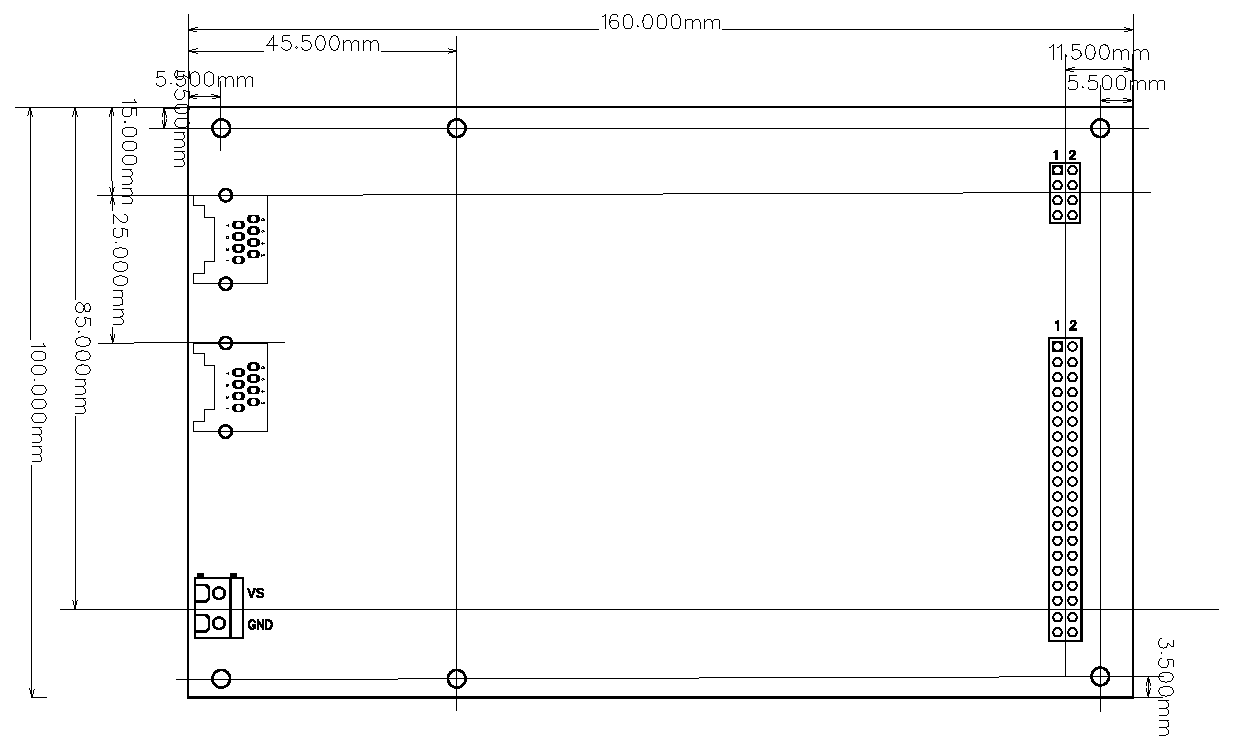
\includegraphics[page=1, scale=0.7]{./Figures/LCS-FP-MAIN-CTRL-10X16.pdf}
    \caption{Board: LCS-FP-MAIN-CTRL-10X16}
    %\label{fig:your-label}
\end{figure}

All boards will have a form factor of 10cm wide and 8, 12, and 16cm long. The figure above shows the 10cm by 16cm board form factor. The main controller board has on the left side the connectors for the LCS bus and the power input. On the right side, there are two connectors toward an extension board. As described before, there are two types of extension boards. The usage of the individual connector pins are described in the upcoming chapter. To ease the hardware schematic development and ensure that all boards fit together, the PCB boards along with their connectors are available as symbols and PCB footprints in the EasyEDA library.

\section{LCS Bus connector}

Every hardware module needs the LCS bus interface to connect to the bus. Some modules may also draw power from this bus. The modules use an RJ45 connector for connecting to the bus. The bus signals can be grouped in several categories. The CAN bus differential lines represent the CAN bus. The VS line is intended for hardware modules with very little power consumptions so that they can directly be powered by the bus. The DCC signal lines are an exact copy of the DCC signal that would go to a track sent out by the DCC signal generating base station. The signal is intended to be routed from the base station to booster nodes, but also to hardware modules that analyze the DCC signal for some action. Finally there is the STOP signal line. This is a wired OR line that allows a simple button along the layout with access to this line to issue a STOP signal. The base station or any nodes interested in the signal can monitor this line. There are the following signal lines.

\begin{longtable}{@{}|l|l|p{0.6\linewidth}|@{}}
    %\caption{Bus Connector Pins}
    \toprule
    \textbf{Pin} & \textbf{Name} & \textbf{Purpose} \\
    \midrule
    \endfirsthead
    \toprule
    \textbf{Pin} & \textbf{Name} & \textbf{Purpose} \\
    \midrule
    \endhead
    \midrule
    \multicolumn{2}{r}{\textit{Continued on next page}} \\
    \midrule
    \endfoot
    \bottomrule
    \endlastfoot
    1 & DCC-Sig-1 & The DCC signal labelled "+" \\
    \midrule
    2 & DCC-Sig-2 & The DCC signal labelled "-" \\
    \midrule
    3 & GND & Common ground \\
    \midrule
    4 & RSV & reserved for future extensions. \\
    \midrule
    5 & RSV & reserved for future extensions. \\
    \midrule
    6 & PWR & The bus supplied 12V power line. This line is intended for devices with very little power consumption to get their power from. Module with high power consumption should connect to its own power supply line. \\
    \midrule
    7 & CAN-L &  Line L of the differential CAN bus signal. \\
    \midrule
    8 & CAN-H &  Line H of the differential CAN bus signal. \\
\end{longtable}

\section{LCS Nodes Extension Board Connector}

For interchangeability of extensions, there is a standardized \textbf{extension board connector} between controller and extensions. Extension boards have a male connector set on the left hand side. Main controller boards will have a female connector on the right hand side. This way main controller and one extension board can be placed next to each other. Like the controller board, extension boards come in different lengths. The following figure shows the 10x16cm board. 

\begin{figure}[htbp]
    \centering
    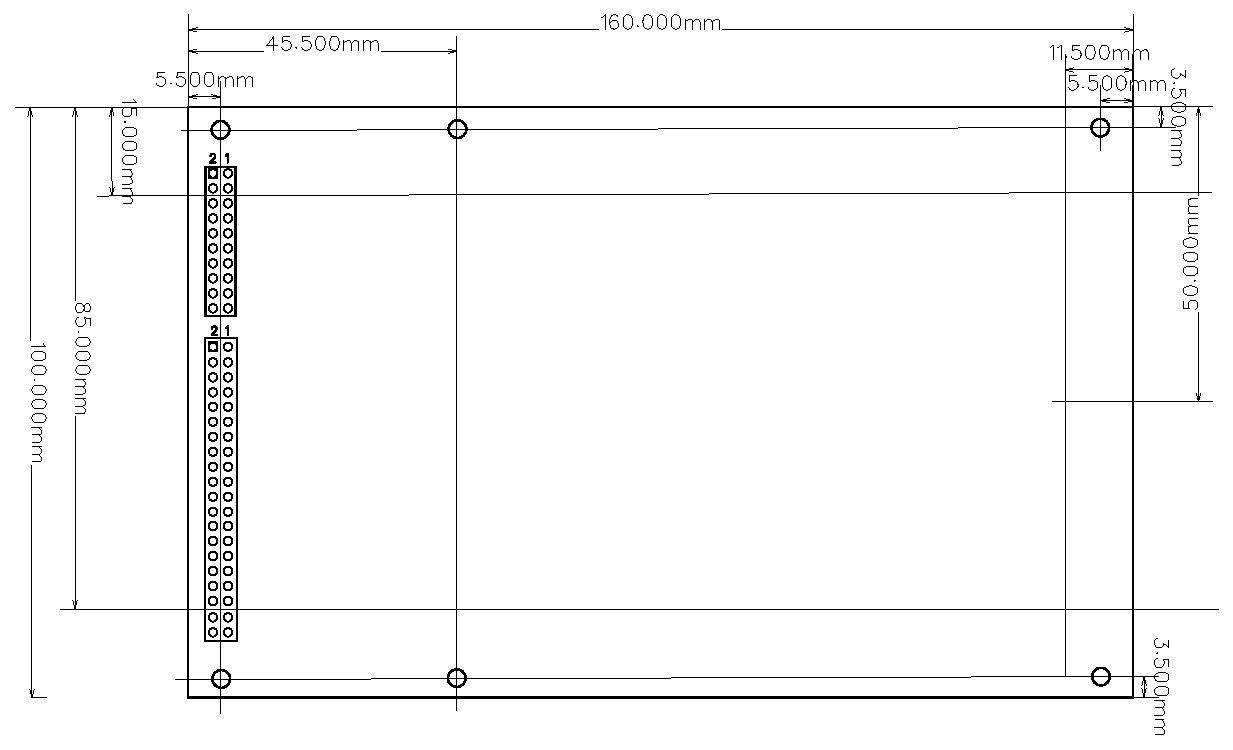
\includegraphics[page=1, scale=0.7]{./Figures/LCS-FP-EXT-L-10X16.pdf}
    \caption{LCS-FP-EXT-R-10X16}
    %\label{fig:your-label}
\end{figure}

Extension boards can also be put into a backplane PCB along with the main controller. This way, more than one extension board can connect to the controller board. The overall concept is very similar to the the shield concept found in the Arduino or Raspberry PI universe, except that we can stack boards, as well as placing two of them next to each other. Up to four extension boards can be connect ed this way.

The I2C interface will be the main communication method between the boards. In fact all current extension boards shown in later chapters use the I2C communication channel. Nevertheless, a rather rich set of outputs from the controller should be available to the extension board for flexibility. There should be ports for digital input and output, analog input, PWM outputs, serial IO and so on. The Raspberry Pi pico offers a great flexibility on assigning function blocks such as an SPI or I2C interface to pins. The extension connector outlined below offers a set of pins which are mapped to the PICO capabilities. The following table shows the connector pin assignments for the communication between a main controller board and extension boards. All boards will have a 40-pin connector organized as 2 rows of 20 pins.

\begin{longtable}{@{}|p{0.1\linewidth}|p{0.1\linewidth}|p{0.1\linewidth}|p{0.1\linewidth}|p{0.4\linewidth}|@{}}
    \caption{Extension Connector} \\
    \toprule
    \textbf{Pin} & \textbf{Name} & \textbf{Pin} & \textbf{Name} & \textbf{Purpose} \\
    \midrule
    \endfirsthead
    \toprule
    \textbf{Pin} & \textbf{Name} & \textbf{Pin} & \textbf{Name} & \textbf{Purpose} \\
    \midrule
    \endhead
    \midrule
    \multicolumn{2}{r}{\textit{Continued on next page}} \\
    \midrule
    \endfoot
    \bottomrule
    \endlastfoot
    1 & \textbf{DCC-1} & 2 & \textbf{DCC-2} & The DCC "+" and "-" signal as generated by the DCC Signal Generator. "+" refers to DCC-1. These pins are typically driven by the base station generating the layout DCC signal.\\
    \midrule
    3 & \textbf{GND} & 4 & \textbf{GND} & Common ground pins. \\
    \midrule
    5 & \textbf{ADC-0} & 6 & \textbf{ADC-1} & Analog input pins. The input is not protected. The analog voltage range is 0 to VCC. \\
    \midrule
    7 & \textbf{GND} & 8 & \textbf{GND} & Common ground pins. \\
    \midrule
    9 & \textbf{DIO-0} & 10 & \textbf{DIO-1} & Plain digital Pins, input or output. The pins are protected. \\
    \midrule
    11 & \textbf{DIO-2} & 12 & \textbf{DIO-3} & Plain digital Pins, input or output. The pins are protected. \\
    \midrule
    13 & \textbf{DIO-4} & 14 & \textbf{DIO-5} & Plain digital Pins, input or output. The pins are protected. \\
    \midrule
    15 & \textbf{DIO-6} & 16 & \textbf{DIO-7} & Plain digital Pins, input or output. The pins are protected. \\
    \midrule
    17 & \textbf{DIO-8} & 18 & \textbf{DIO-9} & Plain digital Pins, input or output. The pins are protected. \\
    \midrule
    19 & \textbf{DIO-10} & 20 & \textbf{DIO-11} & Plain digital Pins, input or output. The pins are protected. \\
    \midrule
    21 & \textbf{GND} & 22 & \textbf{GND} & Common ground pins. \\
    \midrule
    23 & \textbf{BC-0} & 24 & \textbf{BC-1} & Bus Address lines. Up to four extension boards can be connected, the BC pins are used to determine the I2C root address on the I2C extension bus. \\ 
    \midrule
    25 & \textbf{BC-2} & 26 & \textbf{BC-3} & Bus Address lines. Reserved. \\ 
    \midrule
    27 & \textbf{SCL} &  28 & \textbf{SDA} & I2C extension bus channel.  The lines are protected with a serial resistor and there is a pull-up resistor to VCC. \\
    \midrule
    29 & \textbf{RST} & 30 & \textbf{EXT} & RST is reset line. Active Low. EXT is the external interrupt line which be raised from an extension board. Active low. \\
    \midrule
    31 & \textbf{VCC} & 32 & \textbf{VCC} & VCC 5V supply to extension boards. \\
    \midrule
    33 & \textbf{GND} & 34 & \textbf{GND} & Common ground pins. \\
    \midrule
    35 & \textbf{VS} & 36 & \textbf{VS} & Board Input voltage forward. These  connector pins are primarily used by extension boards that need the high power input. Examples  are H-Bridges on such a board or boards that have their power supply circuitry. \\
    \midrule
    37 & \textbf{VS} & 38 & \textbf{VS} & Board Input voltage forward. \\
    \midrule
    39 & \textbf{GND} & 40 & \textbf{GND} & Common ground pins. \\
\end{longtable}  

There are EasyEDA symbols and PCB footprints that offer the connector pins without you going through these details. The appendix contains EasyEDA symbols for the most common board dimensions with the connectors placed in the correct location. A new projects can just start with these EasyEDA symbols.

A key question is how many controller pins are available to an extension board. As said, most of the extension boards would just need the I2C bus to drive the I2C capable ICs on an extension board. However, since there might be rather complex extension boards, the IO pins needed from the controller board to the extension are many and should allow not only for digital IO but also the function blocks inside the controller. The \texttt{DIO-x} pins on the connector map to the GPIO pins of the Raspberry Pi PICO in a way that most of the controller capabilities can be used on an extension board. We will discuss this in more detail in the main controller chapter.

For even more complex extension boards with many connection to the controller board, it is perhaps the better idea to combine a main board with an extension board capabilities to one monolithic board but still keep the extension connector for other not so complex extension boards to attach. 

\section{Track Power Connectors}

In addition to the extension board connector, there is the \textbf{track power connector}. This connector is only used by the base station, block controller and associated extensions. Its purpose is to pass the track power signals from the H-bridges on the base station or block controller ( or booster ) board to the extension boards. This connector is described in more detail in the base station and block controller chapter.

\begin{longtable}{@{}|l|l|p{0.4\linewidth}|@{}}
    \caption{Controller Attributes} \\
    \toprule
    \textbf{Pin} & \textbf{Name} & \textbf{Purpose} \\
    \midrule
    \endfirsthead
    \toprule
    \textbf{Pin} & \textbf{Name} & \textbf{Purpose} \\
    \midrule
    \endhead
    \midrule
    \endfoot
    \bottomrule
    \endlastfoot
    1, 2 & \textbf{GND} & Ground \\
    \midrule
    3, 4 & \textbf{DCC-SIG-B0} & Bridge-0 DCC Signal "+". \\
    \midrule
    5, 6 & \textbf{DCC-SIG-B0} & Bridge-0 DCC Signal "-". \\
    \midrule
    7, 8 & \textbf{DCC-SIG-B1} & Bridge-1 DCC Signal "+". \\
    \midrule
    9, 10 & \textbf{DCC-SIG-B1} & Bridge-1 DCC Signal "-". \\
    \midrule
    11, 12 & \textbf{DCC-SIG-B2} & Bridge-2 DCC Signal "+". \\
    \midrule
    13, 14 & \textbf{DCC-SIG-B2} & Bridge-2 DCC Signal "-". \\
    \midrule
    15, 16 & \textbf{DCC-SIG-B3} & Bridge-3 DCC Signal "+". \\
    \midrule
    17, 18 & \textbf{DCC-SIG-B3} & Bridge-3 DCC Signal "-". \\
    \midrule
    19, 20 & \textbf{GND} & Ground \\
\end{longtable}%

When using all four bridge signal output pairs, each each output pair is rated up to 6 Amps. For high power bridges with up to 6Amps, two pairs can be combined and the number of bridges signals passed on is two.

\section{Controller and Extension Board}

// ??? what to keep here vs. extension patt ?

Controller and Extension boards make up a node. The main controller board will connect via two main bus connectors to an extension board. The pins of the connectors were shown in the previous sections. The following figure depicts how the two boards are connected. There are two basic cases. The first case, shown here, is an extension board that simply is plugged into the connector of the main controller or another extension board.

\begin{figure}[htbp]
    \centering
    \begin{tikzpicture}[scale=1, transform shape]
        \useasboundingbox (0,0) rectangle (15,6);
        \draw[help lines, gray!50, dashed] (0,0) grid(15,6);

        \node at (3.5, 2.5) {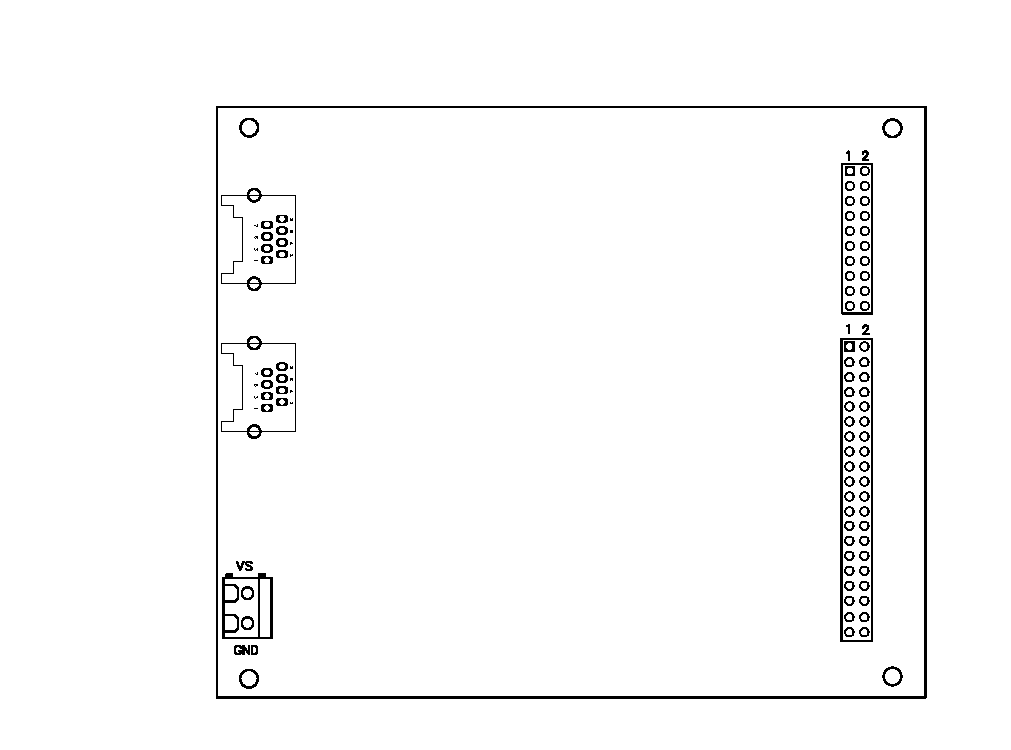
\includegraphics[page=1, width=0.5\textwidth]{./Figures/LCS-FP-MAIN-CTRL-Sketch.pdf}};

        \node at (11.5, 2.5) {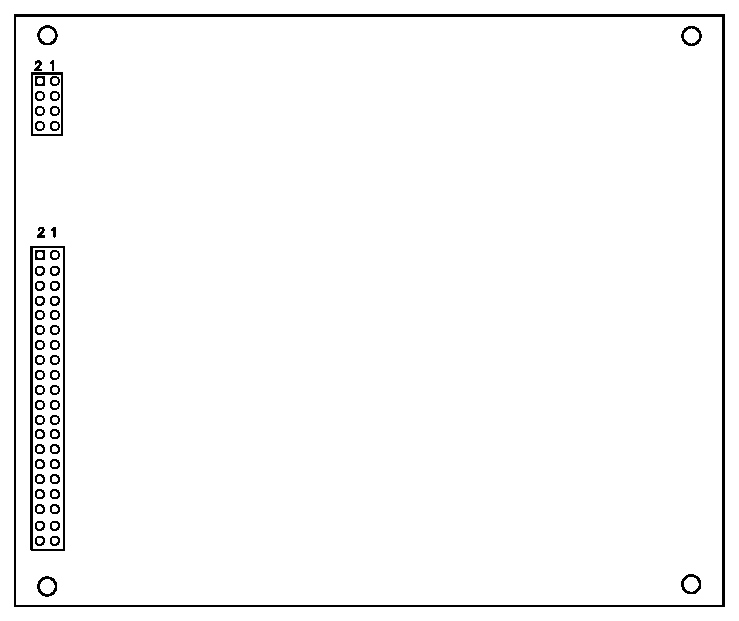
\includegraphics[page=1, width=0.5\textwidth]{./Figures/LCS-FP-EXT-L-Sketch.pdf}};

        \node at (3, 5.5) {\textbf{Main Controller}};
        \node at (11, 5.5) {\textbf{Extension Board}};
        \node at (3.5, 4.3) {Track Bus};
        \node at (3.5, 1.7) {Extension Bus};

        \draw[line width=1mm, gray!40, ->] (5, 3.7) -- (11,3.7);
        \draw[line width=1mm, gray!40, ->] (5,1.7) -- (11,1.7);
    
    \end{tikzpicture}
    \caption{Connecting boards}
    %\label{fig:composite-image}
\end{figure}

Since there are only up to four extension boards supported on one controller, the signal line length is reasonable. For a more compact arrangement, extension boards with only the right hand side connector can be plugged into a backplane style board with the main controller next to it. Nothing else as far as connectivity goes is changed. The appendix on the board design details has the detailed layout of such a board.

\section{Summary}

This chapter introduced the basic ideas behind a hardware module, it connectors and board layout. A key concept is the idea of a common component, the main controller, and extensions that can be connected. Nevertheless, there are good cases for combining a main controller and the extension hardware into one monolithic board. But in any case, the connectors and their purposes stay the same from board to board. While the main controller boards always have the LCS bus and power input on the left side, the extension connector and track line connector on the right, extension boards come in two flavors. 

// ??? add to extension part ...

The first extension board type has male connectors for track line and extension lines on the left side of the board while the second type has not. Both types have female track line and extension line connectors on their right. The first type can just be plugged into the main controller type boards, additional extension boards are simply plugged into the previous extension board. The second extension type is intended for a backplane type design where main controller boards as well as up to four extension board types are plugged into a backplane board. Throughout the chapter to come, you will see how easy boards can be combined using the two connectors lanes and standards behind them. 

Ready for the first hardware work ? All aboard, the train leaves for the next chapter.

